\chapter{Search for invisibly decaying Higgs bosons in Run 1 parked data}
\label{chap:parked}
The parked data, described in \SectionRef{sec:triggers}, used for this analysis was collected using a range of triggers with similar but looser requirements than that used for the prompt data analysis described in the previous chapter. These looser requirements allow areas of phase space which were previously removed by the prompt trigger to be used. However, these regions also have very high levels of \ac{QCD} multijet backgrounds, and require the analysis selection and some background estimation methods to be redesigned compared to the prompt analysis.

%??prkedgains111114.pdf for parked vs prompt limits
%??closure161214update for closure test
%??invupdate081214.pdf for some pileup studies
%??framework synch fwprogress300614.pdf
%??preapproval for source of gain and other good things
%??As above for prompt data analysis but focus on differences and limit setting:
%??New trigger efficiency characterisation, systematic improvements, signal region optimisation, differences in background estimations including options not used
%??lepton and jet pt requirements
\section{Trigger}%??
\label{sec:parkedtrigger}
The parked data trigger varied throughout LHC Run 1. Run 1 was split into 4 ``eras'', A, B, C and D. During era A data was not being parked, so the prompt data is used. The two other triggers used, one for eras B and C, and one for era D, differed from the prompt trigger in that there was no requirement on the \MET present in each event and the jet \pt and \Mjj requirements were looser. The exact values of the trigger selection cuts are summarised in \TableRef{tab:parkedtrig}.

\begin{table}
  \caption{A summary of the requirements of the triggers used for this analysis in each of LHC Run 1's eras. For the jet requirements all triggers require that there is at least one pair of jets in the event satisfying all of the jet requirements listed in this table. All requirements are on \ac{HLT} variables unless stated otherwise.}
  \label{tab:parkedtrig}
  \begin{tabular}{lc|c|c}
    \hline\hline
    \multirow{2}{*}{Variable} & \multicolumn{3}{c}{Cut in era} \\
    \cline{2-4}
    & A & B \& C & D \\
    \hhline{====}
    L1 \MET & \multicolumn{3}{c}{$>40$ \GeV} \\
    \hline
    \METnoMU & $>65$ \GeV & \multicolumn{2}{c}{No requirement} \\
    \hline
    jet \pt of both jets & $>40$ \GeV & $>35$ \GeV & $>30$ \GeV \\
    \hline
    \Mjj & $>800$ \GeV & \multicolumn{2}{c}{$>700$ \GeV} \\
    \hline
    \detajj & \multicolumn{3}{c}{$>3.5$} \\
    \hline
    $\eta_{j1}\cdot\eta_{j2}$ & \multicolumn{3}{c}{$>0$} \\
    \hline
    \hline
  \end{tabular}
\end{table}

As three different triggers are used the measurement of trigger efficiency must be performed separately for each one. Also, the variables used in the trigger are highly correlated with each other. These correlations mean it is important to either only use regions of phase space where the trigger is fully efficient, as was done in the prompt analysis, or to measure the trigger efficiency in a way that accurately models the effect of these correlations. The cuts required to ensure that each trigger is fully efficient throughout the region selected can be ascertained from \FigureRef{fig:prompttrigplots}. As the trigger used in era A is the same as that used for the prompt analysis, no relaxation would be possible if the data from era A is to be used. Era A only accounts for 5\% of the total data, however even if the analysis selection is chosen such that only the loosest trigger is fully efficient the common \ac{L1} \MET requirements in all three triggers mean that only the thresholds on the sub-leading jet's \pt and the \Mjj would be able to be relaxed and it would still be necessary to discard data in the trigger turn on region which is expected to contain signal events. For these reasons several approaches to measuring the trigger efficiency as a function of the values of all variables used in it were investigated.

First, the trigger efficiency was measured three dimensionally as a function of \METnoMU, \Mjj and sub-leading jet's \pt. An example of one of the results of these mearements in one of the bins in \METnoMU for the era B and C, and the era D triggers can be seen in \FigureRef{fig:parked3dtrigeff}. The three variables used were chosen, as the trigger becomes fully efficient very quickly as a function of the $\eta$ related variables, so no parametrisation of the efficiency is necessary. The number and size of the bins was chosen to ensure that sufficient events are present in each bin to prevent the statistical error on the efficiency measurement being larger than the differences between bins. As can be seen from the figure, this leads to very large differences in efficiency between bins, which leads to discontinuities in the \METnoMU, \Mjj and sub-leading jet \pt distributions when the measured efficiency is applied to \ac{MC} events as a weight. This method was therefore not suitable for use in the final analysis.
%trigeff070414.pdf for full 3D binned plot
\begin{figure} 
  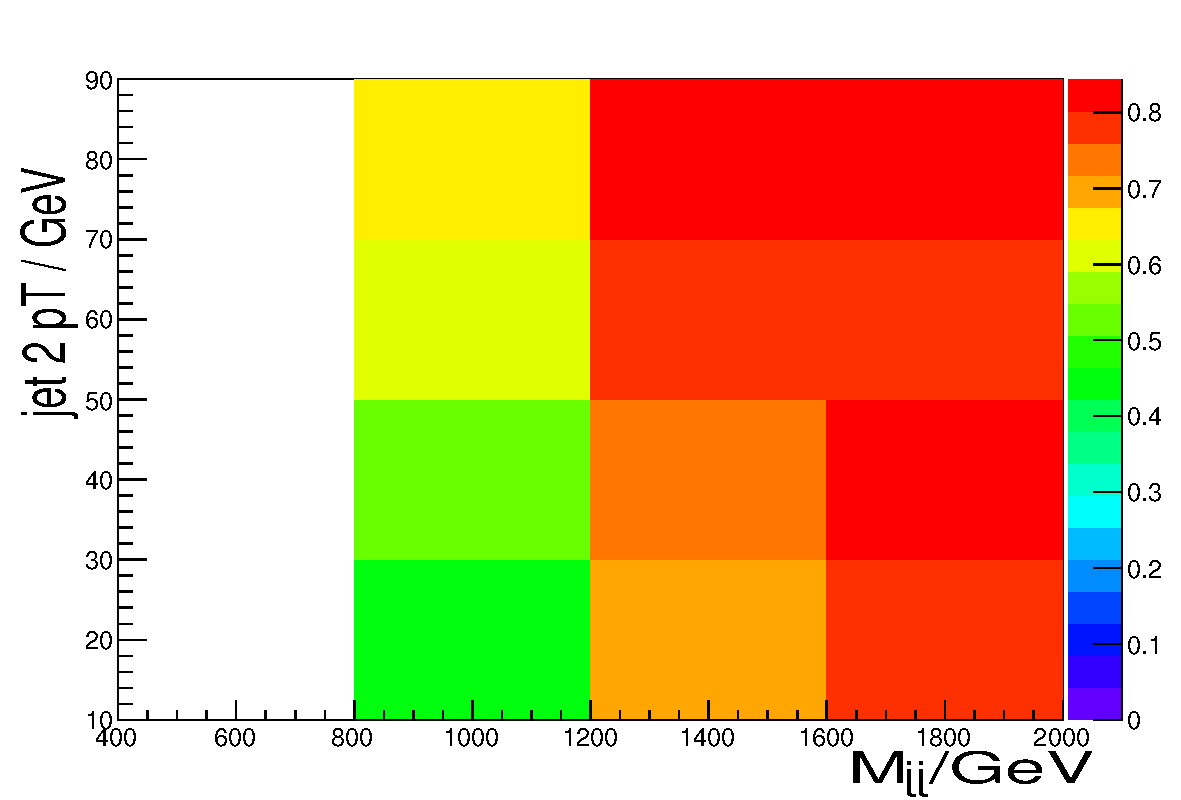
\includegraphics[width=.6\largefigwidth]{plots/parked/HLT_DiJet35_MJJ700_AllJets_DEta3p5_VBFmet120trigeff.pdf}
  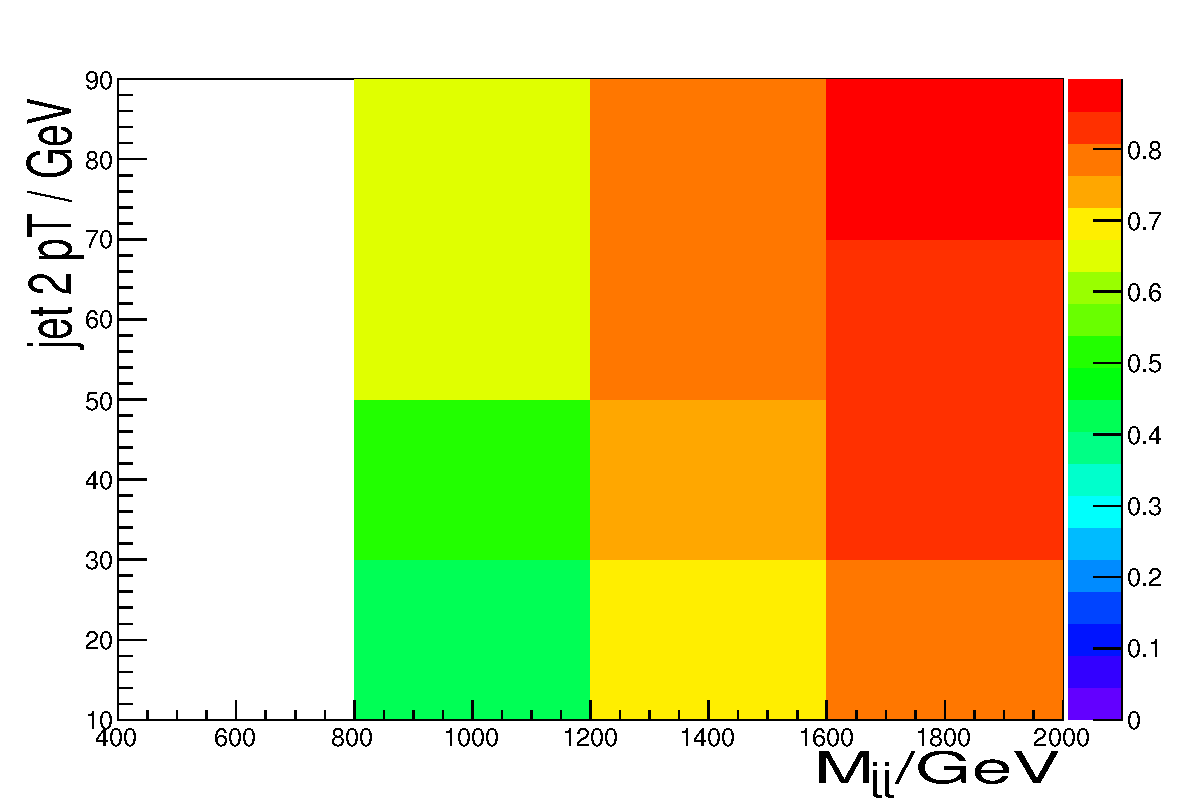
\includegraphics[width=.6\largefigwidth]{plots/parked/HLT_DiJet30_MJJ700_AllJets_DEta3p5_VBFmet120trigeff.pdf}
 \caption{The efficiency for the trigger (color-scale) used in eras B and C (left) and era D (right), as a function of \Mjj and sub-leading jet \pt for events with \METnoMU between 60 and 120 \GeV. The efficiency is measured using a single muon dataset collected with an orthogonal trigger.}
  \label{fig:parked3dtrigeff}
\end{figure}

In order to achieve a smoother trigger efficiency parametrisation, coarse bins in \Mjj and sub-leading jet \pt were chosen and a fit to the \METnoMU efficiency distribution in each bin was performed, using the following function:
\begin{equation}
  \label{eq:parkedtrigfunc}
  f\left(x\right)=\frac{A}{2}\cdot\left(1+ \frac{2}{\sqrt{\pi}}\int_{0}^{\frac{x-B}{\sqrt{C}}}e^{-t^{2}}\mathrm{d}t\right),
\end{equation}
which has a maximum value of A, and is derived from the error function with centre B and width C. The width, maximum and centre of the function are all allowed to float in the fit. The events used in this study were required to have leading jet \pt$>50$ \GeV, $\eta_{j1}\cdot\eta_{j2}<0$ and \detajj$>3.6$ to ensure that there are no inefficiencies due to these variables. The results of these fits for two representative \Mjj and sub-leading jet \pt bins are shown in \FigureRef{fig:parkedtrigeff}, and the results for the remaining bins are shown in \AppendixRef{app:trigeffs}. Some of the plots in the appendix indicate that the parameters of the fit have taken extreme values, or have very large uncertainties. These extreme values and poor fits are mostly due to low numbers of events in the bin, and as described in \SectionRef{sec:parkedsel}, these bins are not used in the final event selection.

\begin{figure}
  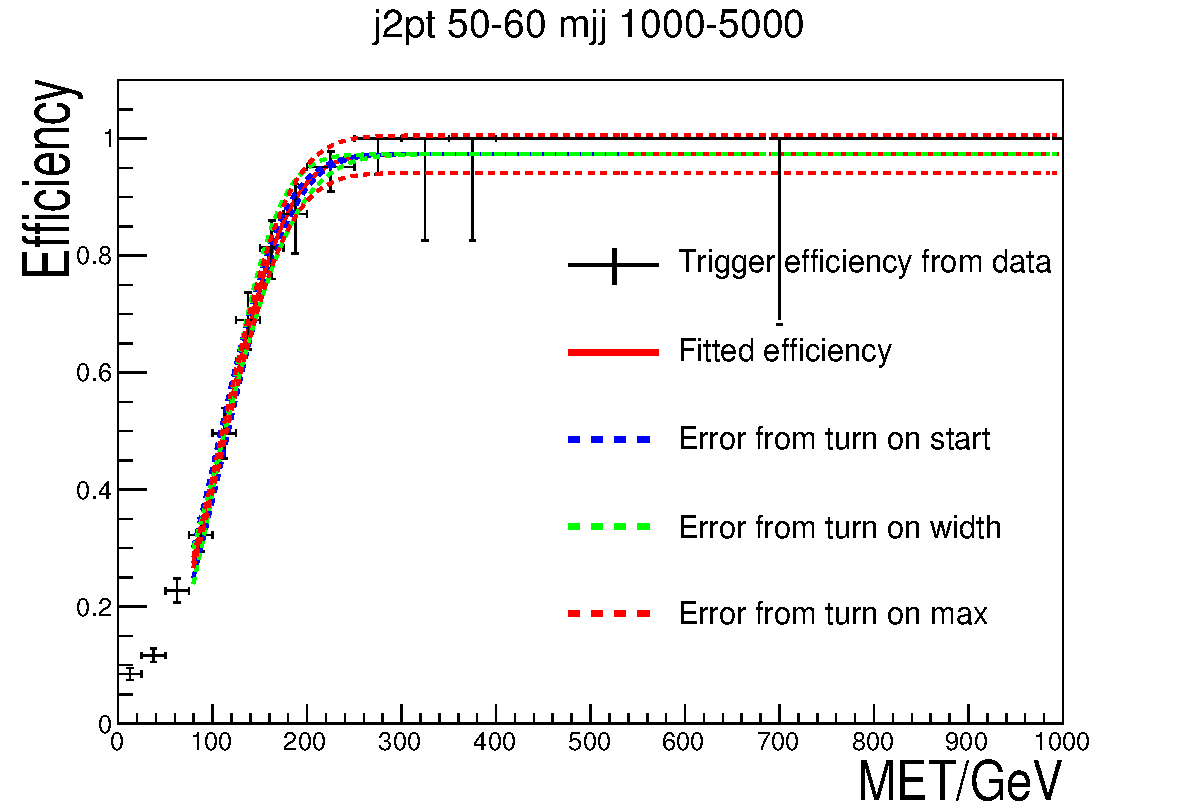
\includegraphics[width=.6\largefigwidth]{plots/parked/trigfitplots/hData_MET_1D_35D.pdf}
  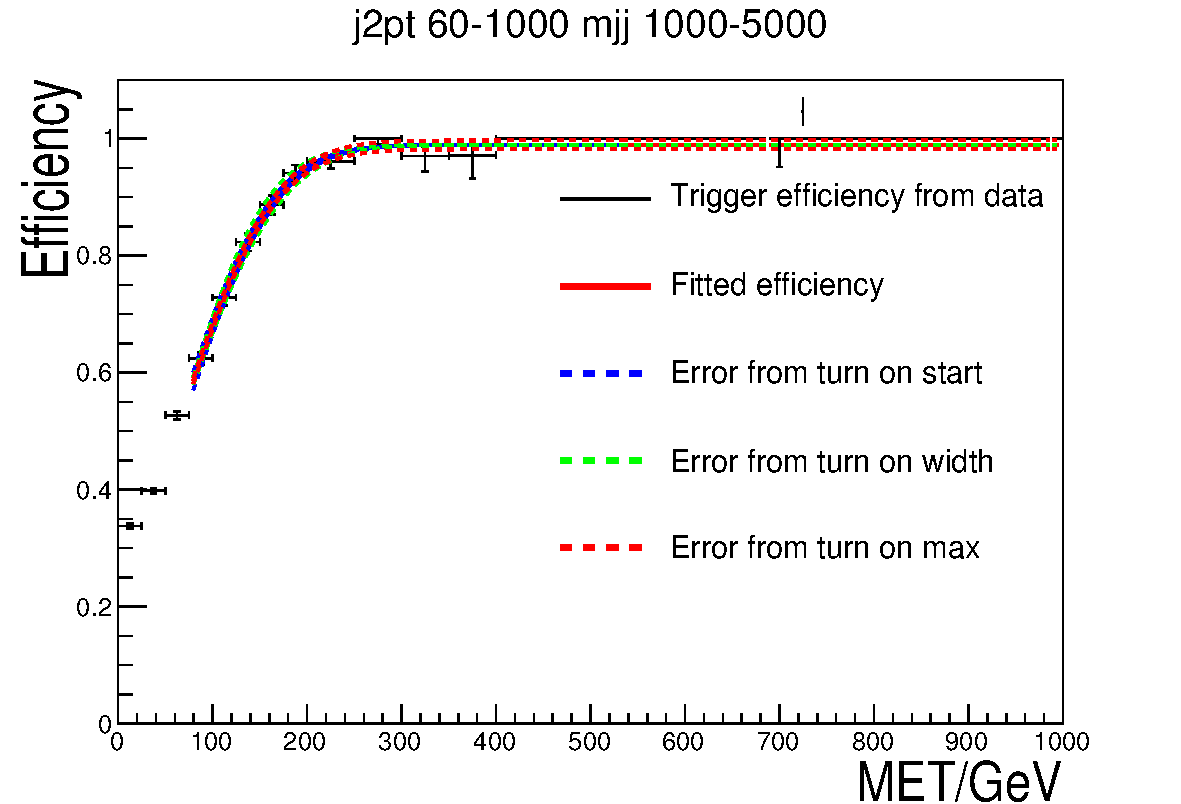
\includegraphics[width=.6\largefigwidth]{plots/parked/trigfitplots/hData_MET_1D_45D.pdf}
  \caption{The results of performing a fit of the function in \EquationRef{eq:parkedtrigfunc} to the efficiency of the trigger used in era D, measured in a sample of single muon events collected with an orthogonal trigger. The dashed bands show the uncertainty on the fit due to each of the three parameters of the fit. The two bins of dijet mass (mjj) and sub-leading jet's \pt (j2pt) shown are those with the two highest numbers of events from the final signal region described in \SectionRef{sec:parkedsel}.}
  \label{fig:parkedtrigeff}
\end{figure}

 The weight applied to each \ac{MC} event is an average of the efficiency found for each of the three triggers weighted as follows by the amount of integrated luminosity recorded using each trigger:
\begin{equation}
  \label{eq:parkedtrigweight}
  w\left(p_{\mathrm{T}j2},\Mjj,\METnoMU\right)=\frac{\sum_{i}\mathcal{L}_{i}\epsilon_{i}\left(p_{\mathrm{T}j2},\Mjj,\METnoMU\right)}{\sum_{i}\mathcal{L}_{i}},
\end{equation}
Where $i$ are the three triggers, $\epsilon_{i}\left(p_{\mathrm{T}j2},\Mjj,\METnoMU\right)$ is the measured efficiency for trigger $i$ as a function of the event's sub-leading jet \pt, \Mjj and \METnoMU, and $\mathcal{L}_{i}$ is the integrated luminosity collected using trigger $i$. The resulting trigger efficiency varies smoothly and leads to no unphysical discontinuities in the distributions of event variables as can be seen from the figures in the remainder of this chapter.

\section{Event selection}%??Possibly restructure into preselection and then optimisation after background estimation section
\label{sec:parkedsel}
As mentioned above a significant challenge of the parked data analysis is that the areas of phase space collected by the parked data triggers but not by the prompt data triggers have very large contributions from \ac{QCD} multijet backgrounds. The \ac{QCD} multijet contribution to \ac{VBF} analyses is very hard to model because whilst the cross-sections for these processes are very high, the probability of any individual event being \ac{VBF}-like is very low, making the number of \ac{MC} events that must be generated prohibitively large. As a result of these difficulties the parked data selection is separated into two stages. The first ``preselection'' stage selects a region of phase space which is not expected to be dominated by \ac{QCD} processes, so that studies could be undertaken into which background estimation methods and final signal region selection lead to the best expected limits. 
%??runcbug101114.pdf sig reg optimisation

\subsection{Preselection}%??
\label{sec:parkedpresel}
The first element of the preselection is motivated by the trigger. The following selection is applied to ensure that the values of all event variables are above the trigger thresholds of all triggers used:
\begin{align}
  \label{eq:parkedprepresel}
  \begin{split}
  \eta_{j1}\cdot\eta_{j2}<0,\,\mathrm{leading\,jet\,}\pt>50 \GeV, \detajj>3.6, \\
  \mathrm{subleading\,jet\,}\pt>40 \GeV, \Mjj>800 GeV, \METnoMU>90\GeV.
  \end{split}
\end{align}
Where $j1$ and $j2$ are the leading and sub-leading \pt jets in the event and are chosen as the \ac{VBF} tag jets. QCD multijet processes still dominate the region defined by this selection, as can be seen in \FigureRef{fig:parkedpresel} top left, where there are a lot more data events than expected from the background \ac{MC} prediction. This difference is due to mismeasured \ac{QCD} multijets events not being adequately modelled by the available \ac{MC} samples. Further pre-selection is therefore necessary to reduce the mismeasured \ac{QCD} multijet background to a level where the large uncertainties on any estimation of its contribution do not have a significant effect on the analysis.

The first variable that is used to achieve this reduction is the \MET significance, \METsig, which is defined as the ratio between \METnoMU and the square root of the sum of the transverse energy of all particles in the event which is an estimate of the statistical error on the \MET. The preselection requires that this variable be greater than 3. The value of this cut was chosen by looking at \FigureRef{fig:parkedpresel} top left and removing the region with the most disagreement between data and \ac{MC}. The resulting region shown in \FigureRef{fig:parkedpresel} top right still does not display good agreement between data and the \ac{MC} prediction, however the disagreement is smaller.

After the cut on \METsig, a requirement that the \METnoMU is not too close to any jets in \phi is made. This requirement is motivated by the high probability for the \MET to be aligned with jets that have been mismeasured. Two variables were investigated, the first was the minimum azimuthal angle difference between either of the two tag jets and the \METnoMU, \jetmetdphileading, and the second was the minimum azimuthal angle difference between any jet with \pt greater than 30 \GeV and the \METnoMU, \jetmetdphi. At a similar signal efficiency the difference between the observed number of events and the \ac{MC} background prediction, which is an indication of the remaining \ac{QCD} multijet background, was found to be 80\% smaller for a cut on \jetmetdphi than a cut on \jetmetdphileading. The same cut on \jetmetdphi was also found to reduce top quark related backgrounds by a factor of two compared to a cut on \jetmetdphileading. We therefore require that \jetmetdphi$>1.0$ for events to pass the preselection.

%contplotsandpresel160914
The \Mjj distribution after the \jetmetdphi cut is shown in \FigureRef{fig:parkedpresel} bottom. Whilst the agreement for large \Mjj is good, it can be seen that the first bin of the distribution, where mismeasured \ac{QCD} multijet events would be expected, due to their not recoiling against another object, shows a significant disagreement. The final cut of the preselection is therefore to require that \Mjj$>1000$ \GeV. In summary the full preselection is as follows:
\begin{equation}
  \label{eq:presel}
  \begin{split}
  \eta_{j1}\cdot\eta_{j2}<0,\,\mathrm{leading\,jet\,}\pt>50 \GeV, \detajj>3.6, \\
  \mathrm{subleading\,jet\,}\pt>40 \GeV, \Mjj>1000 GeV, \METnoMU>90\GeV, \\
  \jetmetdphi>1.0, \METsig>3.0.
  \end{split}
\end{equation}
After defining the preselection the analysis was ``blinded'', i.e. the data observations were not looked at whilst the analysis was being designed.


%AN-14-243
\begin{figure}
  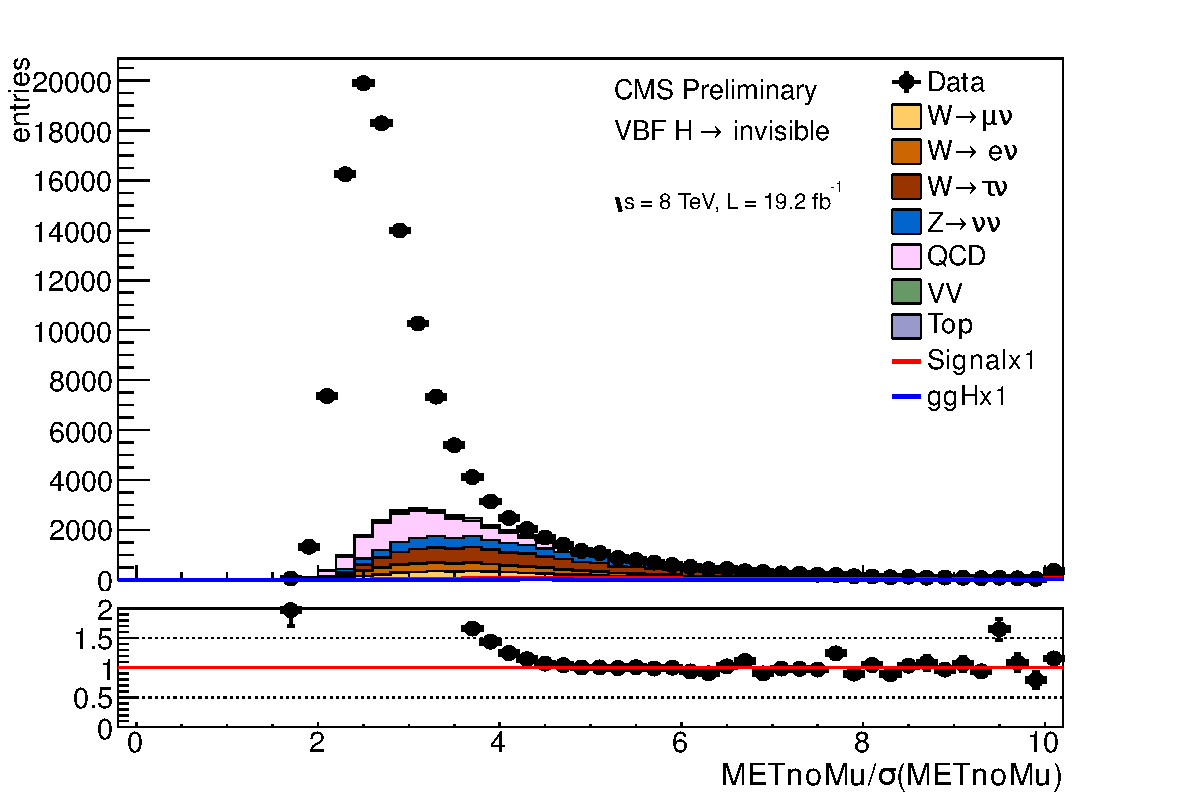
\includegraphics[width=.6\largefigwidth]{plots/parked/AN-14-243-figs/nopreselnunu_metnomu_significance.pdf}
  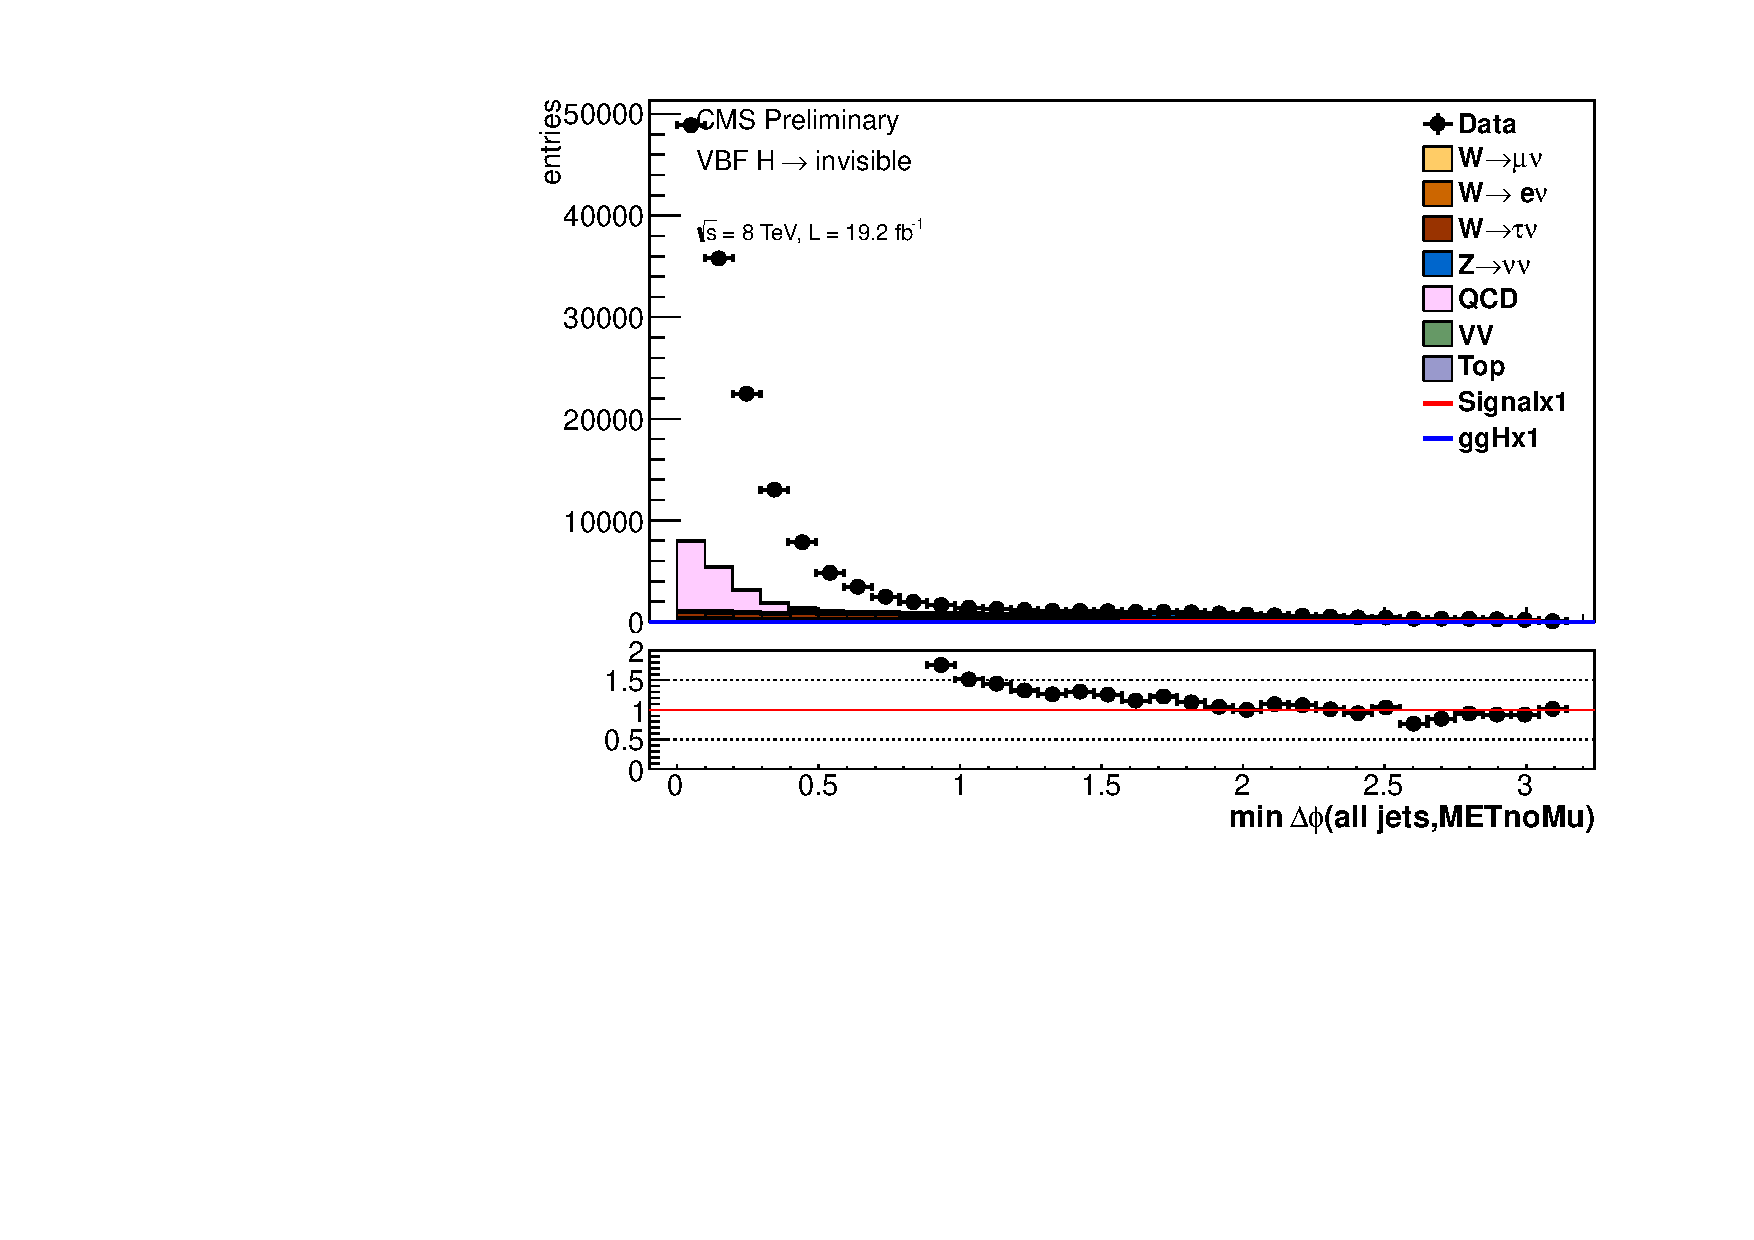
\includegraphics[width=.6\largefigwidth]{plots/parked/AN-14-243-figs/metsigpreselnunu_alljetsmetnomu_mindphi.pdf}

  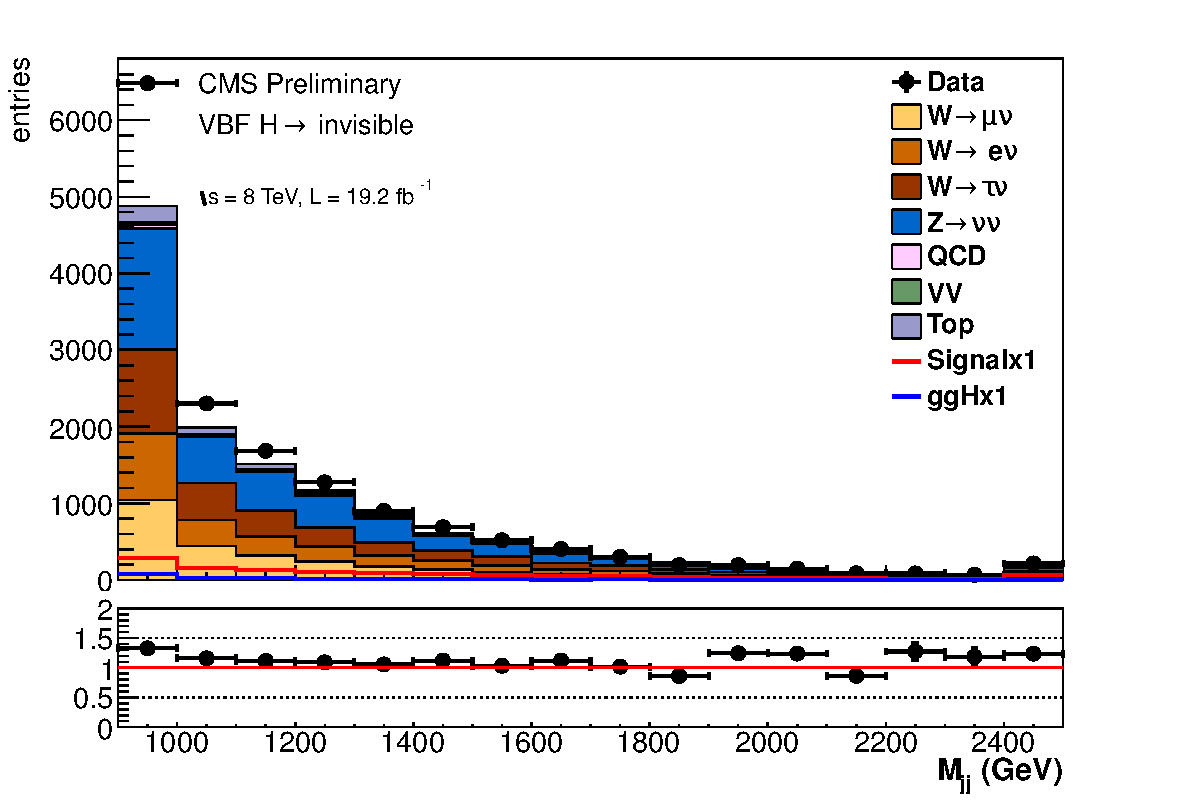
\includegraphics[width=.6\largefigwidth]{plots/parked/AN-14-243-figs/mjj800nunu_dijet_M.pdf}
  \caption{Top left: \METsig after the trigger driven selection described in \EquationRef{eq:parkedprepresel}. Top right: \jetmetdphi after the trigger driven selection and requiring \METsig$>3$. Bottom: \Mjj after the trigger driven selection and requiring \METsig$>3$ and \jetmetdphi$>1$. In all three plots the disagreement between data and the predictions from background \ac{MC} samples are believed to be due to mismeasured \ac{QCD} multijet events which are not well moddelled by the available \ac{MC} samples.}
  \label{fig:parkedpresel}
\end{figure}

%?? and also that any bins in the trigger efficiency parametrisation, described in \SectionRef{sec:parkedtrigger}, with extreme values of the fit parameters or very large uncertainties are not used:


\subsection{Signal region selection}%??
\label{sec:parkedsigsel}


\section{Background estimation}%??                                                                                                                          
\label{sec:parkedbkg}

\subsection{W$\rightarrow e\nu$+jets}%??                                                                                                                    
\label{sec:parkedwenu}

\subsection{W$\rightarrow \mu\nu$+jets}%??                                                                                                                  
\label{sec:parkedwmunu}

\subsection{W$\rightarrow \tau\nu$+jets}%??                                                                                                                 
\label{sec:parkedwtaunu}

\subsection{Z$\rightarrow \nu\nu$+jets}%??                                                                                                                  
\label{sec:parkedznunu}

\subsection{QCD}%??                                                                                                                                         
\label{sec:parkedQCD}

\subsection{Minor backgrounds}%??
\label{sec:parkedminor}

\section{Systematic uncertainties}%??
\label{sec:parkedsyst}
The uncertainty due to the reweighting process used to account for trigger inefficiencies cancels in all data driven background estimates, as a ratio of \ac{MC} event yields is taken. To estimate the size of the uncertainty that should be applied to processes not taken from data driven background, the bin with the largest uncertainties on its fit for each era was chosen. It was then assumed that all bins had this worst-case uncertainty. This resulted in a 2.3\% overall uncertainty on these processes from this effect. Given that this error is smaller than many of the other errors considered, and that the uncertainty on the efficiency in most of the fit bins is significantly lower than this worst case this uncertainty is considered negligible.



\section{Results}%??                                                                                                                                        
\label{sec:parkedresults}
